\documentclass[11pt,a4paper, parskip=half ]{report}
\usepackage[aux]{rerunfilecheck}
\usepackage{polyglossia}
\setmainlanguage{german}
\usepackage[utf8x]{inputenc}
%\usepackage{floatflt}
\usepackage{float}
\floatplacement{figure}{htbp}
\floatplacement{table}{htbp}
\pagestyle{empty}
\usepackage{multicol}
\usepackage{graphicx}
\usepackage{amssymb}
\usepackage{amsmath}
\usepackage{xparse}
\usepackage{braket}
\usepackage{units}
\usepackage[locale=DE,separate-uncertainty=true,per-mode=reciprocal,output-decimal-marker={,},]{siunitx}
\usepackage[section]{placeins}
\usepackage{pdflscape}
\usepackage{expl3}
\usepackage{bookmark}
\usepackage{sidecap}
%Komma als Dezimaltrenner in der mathe Umgebung, um in Umgebungen wie [0, 2] ein Leerzeichen nach dem Komma zu erhalten einfach eins setzen
\usepackage{icomma}
\textwidth16.5cm
\textheight26.5cm
\oddsidemargin0cm \evensidemargin-0.5cm \topmargin-1.5cm
\setlength{\parindent}{0pt}

\renewcommand{\labelenumi}{\alph{enumi})}
\newcommand{\Einheit}[1]{\ensuremath{\,\mathrm{#1}}}
\newcommand{\FracEinheit}[2]{\ensuremath{\,\frac{\mathrm{#1}}{\mathrm{#2}}}}
\newcommand{\difft}{\ensuremath{\,\frac{\mathrm{d}}{\mathrm{d}t}}\,}
\newcommand{\diffpr}{\ensuremath{\,\frac{\partial}{\partial r}}\,}
\newcommand{\diffptheta}{\ensuremath{\,\frac{\partial}{\partial \theta}}\,}
\newcommand{\diffpptheta}{\ensuremath{\,\frac{\partial^2}{\partial \theta^2}}\,}
\newcommand{\diffpphi}{\ensuremath{\,\frac{\partial}{\partial \phi}}\,}
\newcommand{\diffppphi}{\ensuremath{\,\frac{\partial^2}{\partial \phi^2}}\,}
\newcommand{\difftt}{\ensuremath{\,\frac{\mathrm{d}^2}{\mathrm{d}t^2}}\,}
\newcommand{\diffx}{\ensuremath{\,\frac{\mathrm{d}}{\mathrm{d}x}}\,}
\newcommand{\diffxx}{\ensuremath{\,\frac{\mathrm{d}^2}{\mathrm{d}x^2}}\,}
\newcommand{\vek}[2]{\ensuremath{\left( \begin{array}{c}#1\\#2\end{array} \right)}}
\newcommand{\vektor}[3]{\ensuremath{\left( \begin{array}{c}#1\\#2\\#3\end{array} \right)}}
\newcommand{\KleinerAbstand}{\\[5pt]}
\newcommand{\GrosserAbstand}{\\[12pt]}
\newcommand{\NaechsteSeite}{\begin{flushright}\textit{bitte wenden!}\end{flushright}\newpage}
\newcommand{\NaechstesBlatt}{\begin{flushright}\textit{weiter auf zweitem Blatt!}\end{flushright}\newpage}
\graphicspath{{../Bilder/}}
%\hyphenation{}


%%%%%%%%%%%%%%%%%%%%%%%%%%%%%%%%%%%%%
%% Deklarierung eigenere Operatoren%%
%%%%%%%%%%%%%%%%%%%%%%%%%%%%%%%%%%%%%
\DeclareMathOperator{\Div}{div}
\DeclareMathOperator{\Rot}{rot}
%%%%%%%%%%%%%%%%%%%%%%%%%%%%%%%%%%%%%


\begin{document}


\includegraphics[width=\textwidth]{logo_tu_fp.png}
%\GrosserAbstand
\begin{center}
\Large{\textbf{4. \"Ubungsblatt zum Vorkurs Physik - Lösungen}}
\GrosserAbstand
\normalsize
Wintersemester 2020/21 \hfill Prof. Dr. Carsten Westphal\\
\textbf{Für den 22.10.2020} \hfill Prof. Dr. Jan Kierfeld \\
\end{center}

%
%
% * * * * * * * * * * * * * * * * * * * * *
%  AUFGABE 1
% * * * * * * * * * * * * * * * * * * * * *
%
%


\section*{Aufgabe 1: Erstes Mal Taylor-Entwicklung}
  Gegeben ist $f(x) = \sqrt[3]{2x + 2}, \quad x \geq -1$.
  \begin{enumerate}
    \item Bestimmen Sie die ersten zwei Ableitungen der Funktion $f$.
    
    \vspace{20pt}
    \begin{align*}
    f(x) &= (2x + 2)^{1/3} \\ 
    f'(x) &= \frac{1}{3} (2x + 2)^{-2/3} \cdot 2 &= \frac{2}{3} (2x + 2)^{-2/3} \\ 
    f''(x) &= \frac{2}{3} \left(\frac{-2}{3}\right) (2x + 2)^{-2/5} \cdot 2 &= -\frac{8}{9} (2x + 2)^{-2/5} \\ 
    \end{align*}

    \item Stellen Sie das Taylorpolynom $2.$ Grades von $f$ mit Entwicklungspunkt $x_0 = 3$ auf.
    \vspace{20pt}
    \begin{align*}
      T_2(x, x_0) = \sum_{k = 0}^{2} \frac{f^{(k)} (x_0)}{k!} (x - x_0)^k = f(x_0) + f'(x_0)(x-x_0) + \frac{f''(x_0)}{2}(x - x_0)^2 
      \end{align*}

      Funktionen auswerten: 
      \begin{align*}
        f(3) &= \sqrt[3]{8} = 2 \\
        f'(3) &= \frac{2}{3} (\frac{1}{\sqrt[3]{8}})^2 = \frac{2}{3 \cdot 4} = \frac{1}{6} \\
        f''(3) &= -\frac{8}{9} (\frac{1}{\sqrt[3]{8}})^5 = -\frac{8}{9 \cdot 32} = - \frac{1}{36} \\
          T_2(x, 3) &= 2 + \frac{1}{6}(x-3) - \frac{1}{72}(x - 3)^2 \\
          \end{align*} 

          \begin{figure}
            \centering
            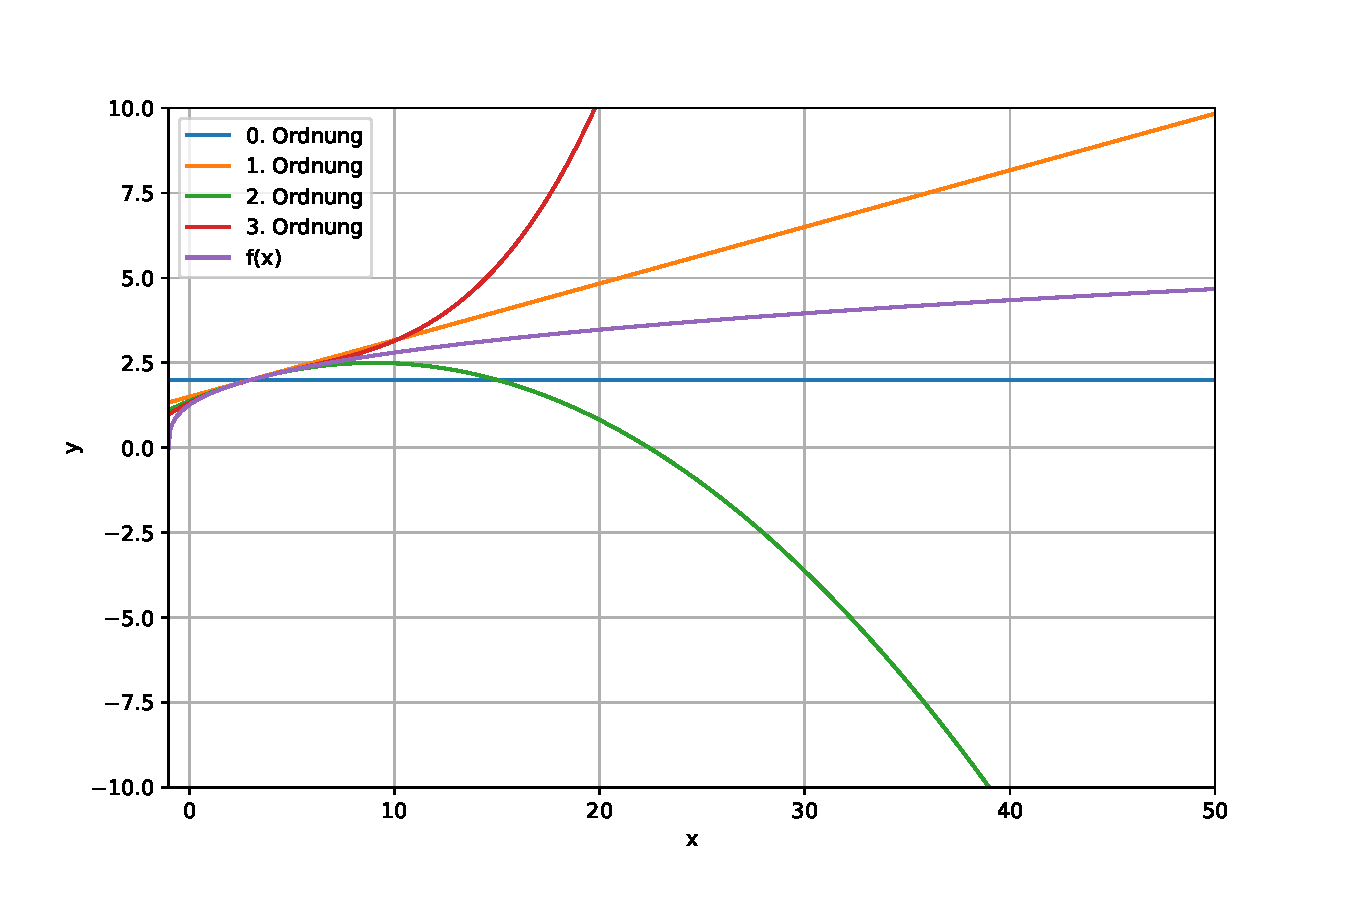
\includegraphics[width=0.8\textwidth]{./Aufgabe_1.pdf}
            \caption{Taylor-Entwicklungen bis zur 3. Ordnung zur Funktion $\sqrt[3]{2x+2}$ mit $x\geq -1$.}
            \label{fig:feynman2}
          \end{figure}
  \end{enumerate}



  \section*{Aufgabe 2: Von Taylor-\textit{Entwicklung} zu Taylor\textit{reihe}}
  Berechnen Sie alle Ableitungen $f^{(n)}$ mit $n = 0, 1, 2, ...$ der Funktion $f$ und geben Sie damit die Taylorreihe für $f$ mit Entwicklungspunkt $x_0 = 0$ an,  
  \begin{enumerate}
    \item $f(x) = \sin(3x), \,\, x \in \mathbb{R}$, 
    
    \vspace{20pt}
    \begin{align*}
    f^{(0)}(x) &= \sin(3x) \\
    f'(x) &= 3 \cdot \cos(3x) = \sin(3x + \frac{\pi}{2}) \\
    f''(x) &= 3^2 \cdot \sin(3x + 2 \frac{\pi}{2}) \\
    f^{(k)}(x) &= 3^k \sin(3x + k \frac{\pi}{2}) \\
    f(x) &= \sin(3x) = \sum_{k = 0}^{\infty} \frac{f^{(k)}(0)}{k!} x^k = \sum_{k = 0}^{\infty} \frac{3^k sin(k \frac{\pi}{2})}{k!} x^k = \sum_{k = 0}^{\infty} \frac{3^{2k+1}}{(2k+1)!} (-1)^k x^{2k+1} \\
    \end{align*}

    \begin{figure}
      \centering
      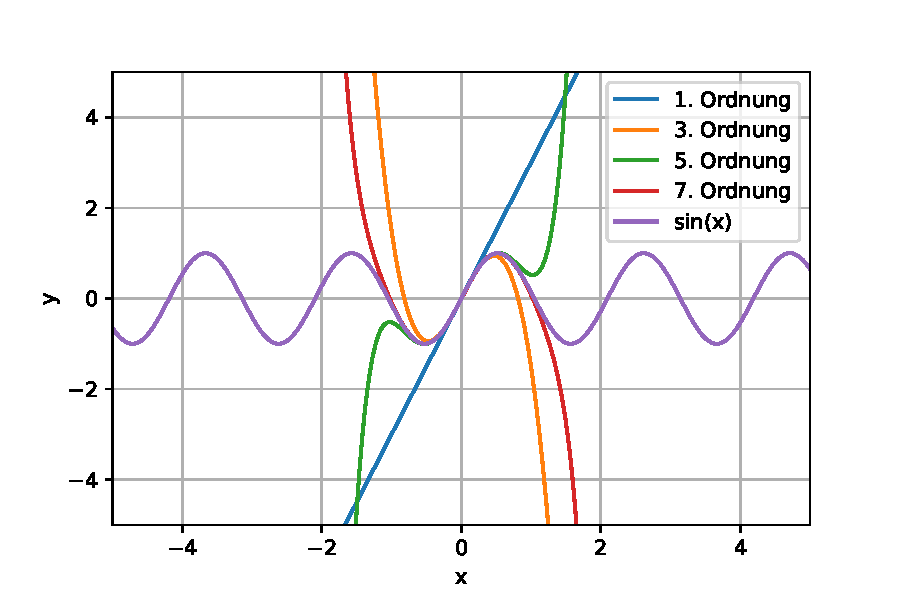
\includegraphics[width=0.8\textwidth]{./Aufgabe_2a.pdf}
      \caption{Taylor-Entwicklungen bis zur 3. Ordnung zur Funktion $\sqrt[3]{2x+2}$ mit $x\geq -1$.}
      \label{fig:feynman2}
    \end{figure}

    \item $f(x) = \sqrt{1+x}, \,\,|x| \leq 1$.
    
    \vspace{20pt}
    \begin{align*}
    f^{(0)}(x) &= (1+x)^{\frac{1}{2}} \\
    f'(x) &= \frac{1}{2} (1+x)^{\frac{1}{2} -1} \\
    f''(x) &= \frac{1}{2} \left(\frac{1}{2} -1\right) (1+x)^{\frac{1}{2} -2} \\
    f^{(k)}(x) &= \frac{1}{2} \left(\frac{1}{2} -1\right) \dots \left(\frac{1}{2} - k + 1\right) (1+x)^{\frac{1}{2} - k} = k! {\frac{1}{2}\choose k} (1 + x)^{\frac{1}{2} - k}\\
    f(x) &= \sum_{k=0}^{\infty} \frac{f^{(k)}(0)}{k!} x^k = \sum_{k=0}^{\infty} {\frac{1}{2}\choose k} x^k \\
    \end{align*}

    \begin{figure}
      \centering
      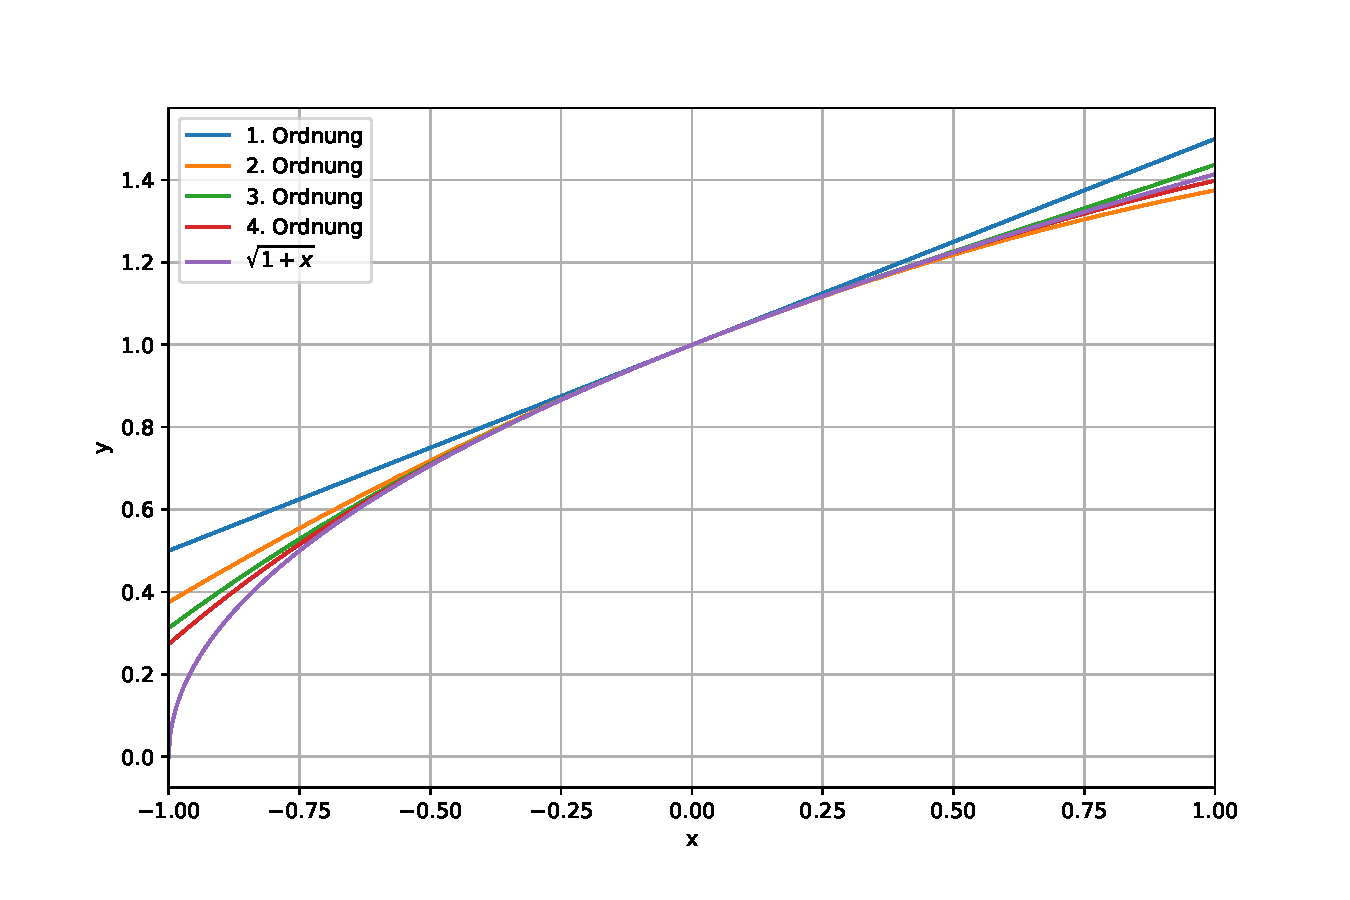
\includegraphics[width=0.8\textwidth]{./Aufgabe_2b.pdf}
      \caption{Taylor-Entwicklungen bis zur 3. Ordnung zur Funktion $\sqrt[3]{2x+2}$ mit $x\geq -1$.}
      \label{fig:feynman2}
    \end{figure}

  \end{enumerate}

  \section*{Aufgabe 3: Taylor-Entwicklung die Zweite}
  Bestimmen Sie das Taylorpolynom dritten Grades der Funktion $f(x) = e^{\sin(x)}$ im Entwicklungspunkt $x_0 = 0$.  
  
  
  \vspace{20pt}
  Weg 1:
  \begin{align*}
  f^{(0)}(x) &= e^{\sin(x)}, f(0) = 1 \\ 
  f'(x)      &= e^{\sin(x)} \cdot \cos(x), f'(0) = 1 \\
  f''(x)     &= (e^{\sin(x)} \cdot \cos^2(x)) + (e^{\sin(x)} \cdot (-\sin(x)), f'(0) = 1 \\
  f'''(x)    &= e^{\sin(x)} \cdot \cos^3(x) + e^{\sin(x)} \cdot 2 \cos(x) (-\sin(x)) + e^{\sin(x)} \cos(x)\cdot (-\sin(x)) + e^{\sin(x)}(-cos(x)) , \\
  f'''(0) &= 1 - 1 = 0 \\
  T_3 (x, 0) &= 1 + x + \frac{1}{2} x^2 \\
  \end{align*}

  Weg 2: 

  Taylor-Reihe der e-Funktion bei $x_0 = 0$: $e^x = 1 + x + \frac{x^2}{2} + \frac{x^3}{6} + \dots$

  Taylor-Reihe des Sinus $x_0 = 0$: $ \sin(x) = x - \frac{x^3}{6} + \dots$ 
  \begin{align*}
  e^{\sin{x}} &= 1 + \left(x - \frac{x^3}{6}\right) + \frac{1}{2} \left(x - \frac{x^3}{6}\right)^2 + \frac{1}{6} \left(x - \frac{x^3}{6}\right)^3 \\
  &= 1 + x + \frac{x^3}{6} + \frac{1}{2} \left(x^2 - \frac{2 x^4}{6} + \frac{x^6}{36}\right) + \frac{1}{6} \left(x^3 - 3 x^2 \left(\frac{x^3}{6}\right) + 3 x \left(\frac{x^3}{6}\right)^2 - \left(\frac{x^3}{6}\right)^3\right) \\
  &= 1+ x + \frac{x^2}{2} -\frac{x^3}{6} + \frac{x^3}{6} - \frac{x^4}{6} - \frac{x^5}{3} + \frac{x^6}{72} - \frac{x^9}{6^4} \\ 
  &= 1 + x + \frac{x^2}{2} + \dots \\
  \end{align*}

  \begin{figure}
    \centering
    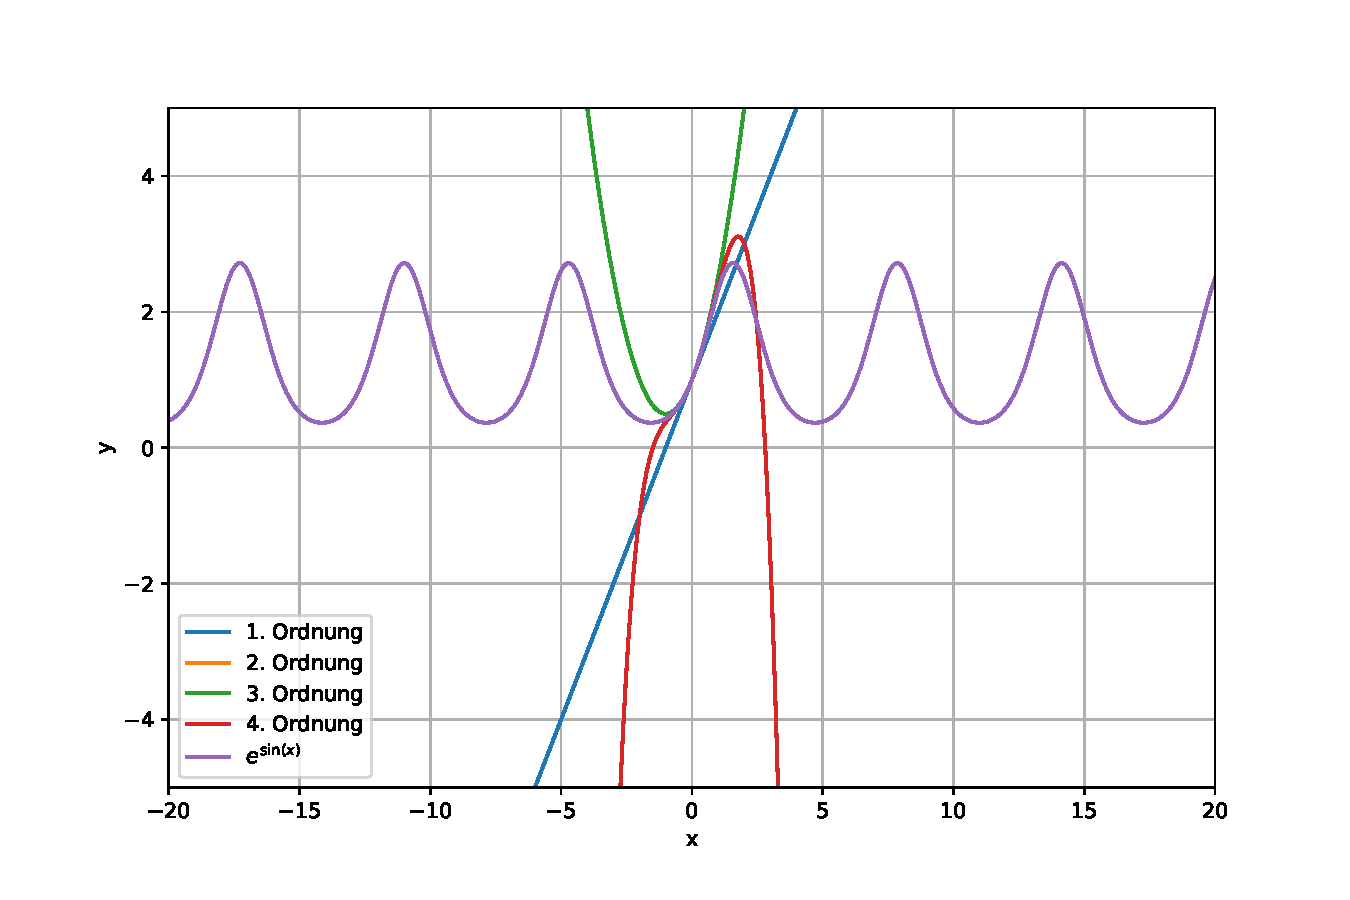
\includegraphics[width=0.8\textwidth]{./Aufgabe_3.pdf}
    \caption{Taylor-Entwicklungen bis zur 3. Ordnung zur Funktion $\sqrt[3]{2x+2}$ mit $x\geq -1$.}
    \label{fig:feynman2}
  \end{figure}

  \section*{Aufgabe 4:  Taylor-Entwicklung die Letzte}
  Bestimmen Sie das Taylorpolynom dritten Grades der Funktion \begin{enumerate}
    \item $f(x) = \sin(x)$ mit $x_0 = 0$,
    
    \vspace{20pt}
  \begin{align*}
  f^{(0)}(x) &= \sin(x), \qquad &f(0) = 0 \\ 
  f'(x)      &= \cos(x), \qquad &f'(0) = 1 \\
  f''(x)     &= -\sin(x), \qquad &f'(0) = 0 \\
  f'''(x)    &= -\cos(x), \qquad &f'''(0) = -1 \\
  f^{4}(x)    &= \sin(x), \qquad &f^{4}(0) = 0 \\
  f^{5}(x)    &= \cos(x), \qquad &f^{5}(0) = 1 \\
  T_5 (x, 0) &= x - \frac{1}{6} x^3 + \frac{1}{120} x^5  &\\
  \end{align*}

  \begin{figure}
    \centering
    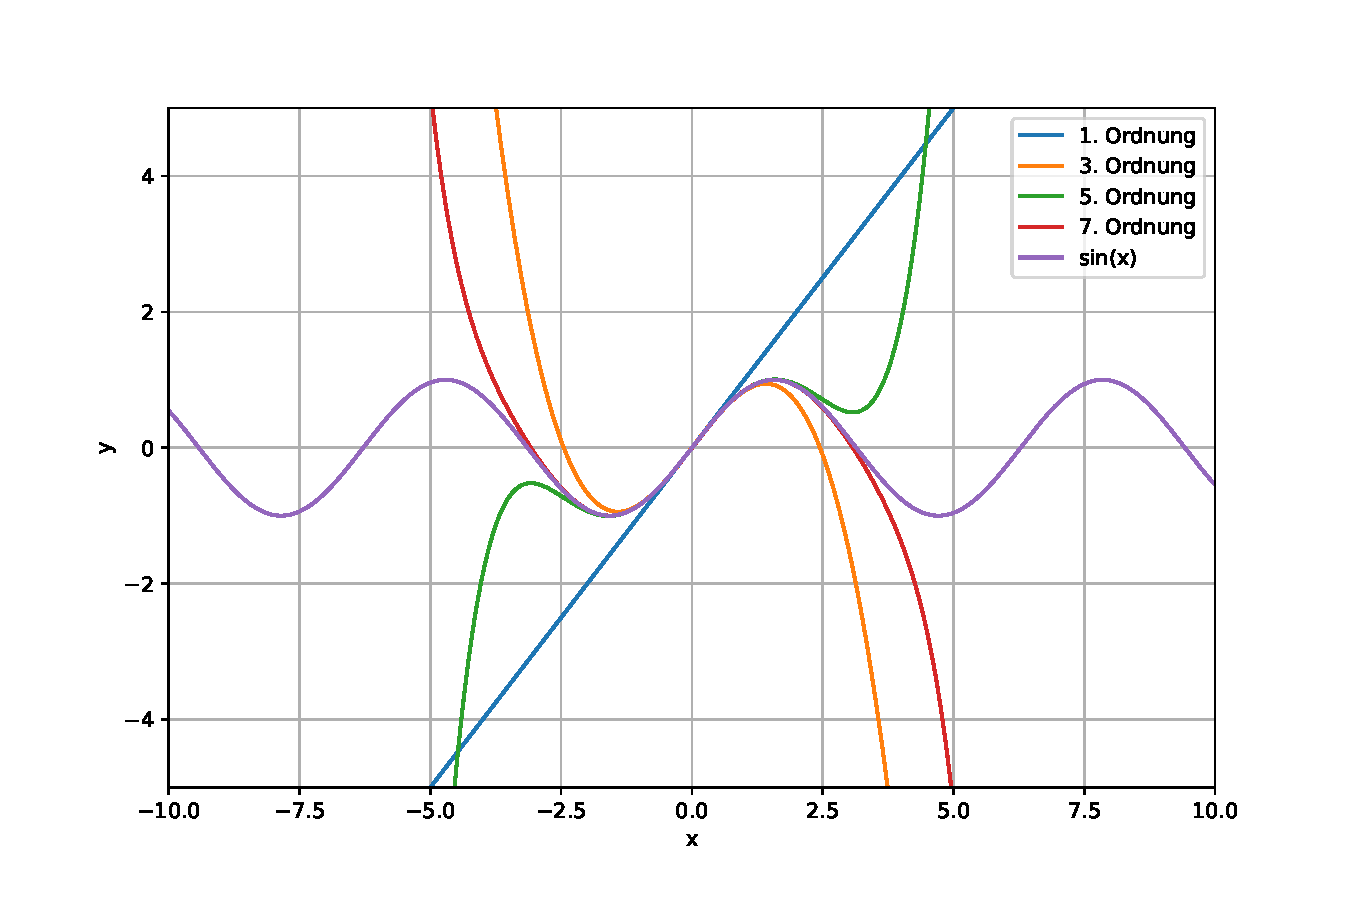
\includegraphics[width=0.8\textwidth]{./Aufgabe_4a.pdf}
    \caption{Taylor-Entwicklungen bis zur 3. Ordnung zur Funktion $\sqrt[3]{2x+2}$ mit $x\geq -1$.}
    \label{fig:feynman2}
  \end{figure}

    \item $f(x) = x \ln(x)$ mit $x_0 = 1$. 
    
    \vspace{20pt}
    \begin{align*}
    f^{(0)}(x) &= x \ln(x), \qquad f(1) = 0 \\ 
    f'(x)      &= \ln(x) + 1, \qquad f'(0) = 1 \\
    f''(x)     &= \frac{1}{x}, \qquad f'(0) = 1 \\
    f'''(x)    &= -\frac{1}{x^2} , \qquad f'''(0) = -1 \\
    T_3 (x, 1) &= (x -1) + \frac{1}{2!} (x-1)^2 - \frac{1}{6} (x-1)^3 \\
    \end{align*}

    \begin{figure}
      \centering
      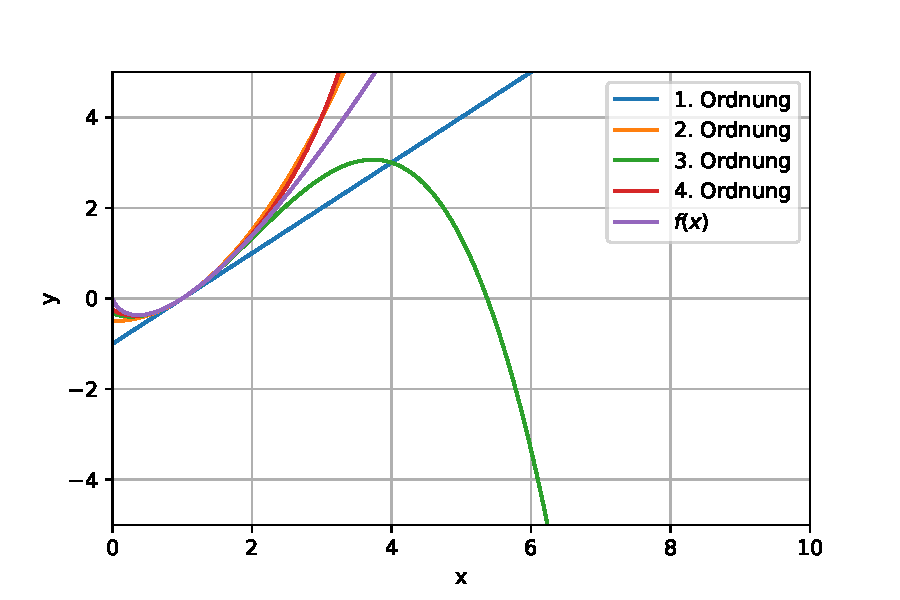
\includegraphics[width=0.8\textwidth]{./Aufgabe_4b.pdf}
      \caption{Taylor-Entwicklungen bis zur 3. Ordnung zur Funktion $\sqrt[3]{2x+2}$ mit $x\geq -1$.}
      \label{fig:feynman2}
    \end{figure}

  \end{enumerate}


  \section*{Aufgabe 5: Kurvendiskussion}
\begin{enumerate}
  \item Bestimmen Sie die Extrempunkte der Funktion f mit $f(x) = e^{2x} + e^{-x}$.
  \vspace{20pt}
  \\Bestimmung der Ableitungen:	$f^{\prime}(x) =  2e^{2x} - e^{-x}$, $f^{\prime\prime}(x) =  4e^{2x} + e^{-x}$	(immer größer Null)\\
	Notwendige Bedingung für einen Extrempunkt:\\  
			$f^{\prime}(x) = 0	\Leftrightarrow  2e^{2x} - e^{-x} = 0 |\cdot e^x  	\Leftrightarrow 2e^{3x} – 1 = 0  \Leftrightarrow     2e^{3x} = 1
			\Leftrightarrow x= \frac{1}{3} \ln(0.5) = -0.231$\\				
	Da f‘‘ > 0 (linksgekrümmt), liegt ein Tiefpunkt vor:	Tiefpunkt T(-0.231|2.52) 

  \item Bestimmen Sie den Wendepunkt der Funktion f mit $f(x) = (x-1)\cdot e^x$.
  \vspace{20pt}
  \\Bestimmung der Ableitungen:  $f^{\prime}(x) = e^x + (x-1)\cdot e^x = (1+x-1)\cdot e^x = x\cdot e^x$, $f^{\prime\prime}(x) = e^x + x\cdot e^x = (x+1)\cdot e^x$	
  \\Notwendige und hinreichende Bedingung für einen Wendepunkt:  
  \\$f^{\prime\prime}(x) = 0	\Leftrightarrow   (x +1)\cdot e^x = 0   \Leftrightarrow x = -1$
  \\$f^{\prime\prime}(0) = 1> 0$, $f^{\prime\prime}(-2) = -e^{-2}< 0   \Rightarrow$ VZW von f′′ von + nach - an der Stelle \num{-1}	
  \\Wendepunkt W(-1|-0.736) 	

\end{enumerate}

\section*{Aufgabe 6: Und weil's so schön war Kurvendiskussion}
\begin{enumerate}
  \item Die Funktion f  hat das nebenstehende Schaubild und die	Funktionsgleichung $f(x) = a\cdot e^x + b$ mit $(a,b \in \mathbb{R})$. Bestimmen Sie die Werte von a und b. Tipp: Betrachten Sie den Verlauf der Funktion.
  \begin{figure}
    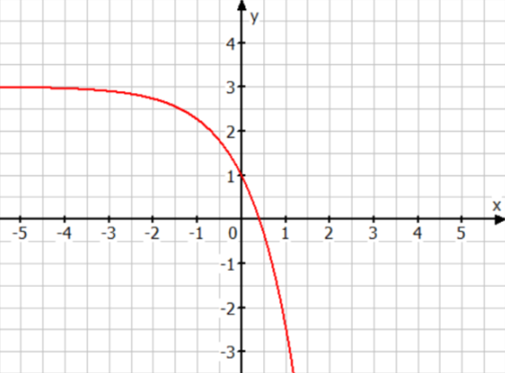
\includegraphics{media/Bild1.png}
  \end{figure}
  \vspace{20pt}
  \\Betrachte Asymptotik des Graphen: mit $\lim_{x\rightarrow\infty} e^{-x} = 0 \Rightarrow b = 3$.
  \\Aus f(0) = 1 folgt a = -2.	
  \item Gegeben sind die Funktionen f und g mit $f(x) = \frac{1}{1-x}+3$ und $g(x)=-\frac{1}{1+x}$.	Geben Sie die waagrechte Asymptote der Funktion f an und bestimmen Sie die Stelle, an der f und g  die gleiche Steigung haben.
  \vspace{20pt}
  \\Betrachte Verhalten für $+\infty$ und $-\infty$ $\Rightarrow$ f(x) hat die waagrechte Asymptote y = 3.
  \\Bestimmung der Ableitungen:	
  \\$f(x) = (1-x)^{-1}+3$, $f^{\prime}(x) = (1-x)^{-2} = \frac{1}{(1-x)^2}$ 
  \\$g(x) = -(1+x)^{-1}$, $g^{\prime}(x) = (1+x)^{-2} = \frac{1}{(1+x)^2}$      
  \\Ableitungen gleichsetzen:
  \\$f^{\prime}(x) = g^{\prime}(x)   \Leftrightarrow 	(1+x)^2 = (1-x)^2 \Leftrightarrow 1+2x+x^2 = 1-2x+x^2 \Leftrightarrow 2x = -2x \Leftrightarrow x = 0$	

\end{enumerate}
 

\end{document}
